\input{main.tex}
\begin{document}
\title{ESPACES EUCLIDIENS}
\author{B. Landelle}
\date{}
\maketitle

\tableofcontents

\section*{I Adjoint d'un endomorphisme}


% Source image: page_002.png

\section{Rappels}

On appelle espace euclidien un espace préhilbertien réel de dimension finie. Dans E espace euclidien, pour tout $x \in E$, on a

\[ E = F \oplus F^\perp \quad \text{et} \quad (F^\perp)^\perp = F \]

Il existe une base orthonormée de E. Soit $\left(e_i\right)_{i=1 \dots n}$ une base orthonormée de E. Pour $x \in E$, on a $x = \sum_{i=1}^n x_i e_i$. Pour $(x, y) \in E^2$, notant $x = \sum_{i=1}^n x_i e_i$ et $y = \sum_{i=1}^n y_i e_i$ et $x = \text{mat}_{\mathbb{R}}$.

Pour $x = \text{mat}_{\mathbb{R}}$, on a

\[ (x, y) = \sum_{i=1}^n x_i y_i = x^T y = (X, Y) \quad \text{et} \quad \|x\|_2 = \sqrt{\sum_{i=1}^n x_i^2} = \sqrt{X^T X} = \|X\|_2 \]

Pour $u \in \mathcal{L}(E)$ et $A = \text{mat}_u = (a_{i, j})_{1 \leq i, j \leq n}$, on a

\[ \forall (i, j) \in [1, n]^2 \quad a_{i, j} = \langle e_i, u(e_j) \rangle \quad \text{et} \quad (x, u(y)) = X^T A Y = \sum_{i=1}^n \sum_{j=1}^n x_i y_j a_{i, j} \]

Dans tout ce qui suit, l'ensemble E désigne un espace euclidien. Les espaces $\mathbb{R}^n$ et $M_{n, 1}(\mathbb{R})$ sont munis de leurs structures euclidiennes canoniques et on confond vecteur de $\mathbb{R}^n$ et matrice colonne de $M_{n, 1}(\mathbb{R})$.

\section{Adjoint d'un endomorphisme}

\subsection{Définition}

\textbf{Théorème 1 (Théorème de représentation de Riesz).}

\[ \forall \varphi \in \mathcal{L}(E, \mathbb{R}) \quad \exists ! a \in E \quad \forall x \in E \quad \varphi(x) = \langle a, x \rangle \]

Démonstration. L'application $\Phi : E \to \mathcal{L}(E, \mathbb{R})$, $a \mapsto (x \mapsto \langle a, x \rangle)$ est linéaire injective entre deux espaces de même dimension donc est un isomorphisme.

Remarque : L'espace $\mathcal{L}(E, \mathbb{R})$ des formes linéaires de E est appelé dual de E et habituellement noté $E^*$.

\textbf{Théorème 2.} Soit $u \in \mathcal{L}(E)$. Il existe un unique endomorphisme $u^* \in \mathcal{L}(E)$ vérifiant

\[ \forall (x, y) \in E^2 \quad (u(x), y) = (x, u^*(y)) \]

Démonstration. Soit $y \in E$. D'après le théorème de Riesz appliqué à la forme linéaire $x \mapsto \langle u(x), y \rangle$, on dispose d'un unique $u^*(y) \in E$ tel que

\[ \langle u(x), y \rangle = \langle x, u^*(y) \rangle \quad \forall x \in E \]

ce qui prouve l'existence d'une unique application $u^* : E \to E$ vérifiant la relation attendue.
Soient $y_1, y_2 \in E$ et $x \in E$. Alors

\[ \langle u(x), y_1 + y_2 \rangle = \langle u(x), y_1 \rangle + \langle u(x), y_2 \rangle = \langle x, u^*(y_1) \rangle + \langle x, u^*(y_2) \rangle = \langle x, u^*(y_1) + u^*(y_2) \rangle \]

donc $u^*(y_1 + y_2) = u^*(y_1) + u^*(y_2)$. De même, pour tout $x \in E$ et $\lambda \in \mathbb{R}$, on a

\[ \langle u(x), \lambda y \rangle = \lambda \langle u(x), y \rangle = \lambda \langle x, u^*(y) \rangle = \langle x, \lambda u^*(y) \rangle \]

d'où $u^*(\lambda y) = \lambda u^*(y)$.

B. Landelle

\textbf{Définition 1.} Soit $u \in \mathcal{L}(E)$. L'endomorphisme $u^*$ est appelé endomorphisme adjoint de $u$.
\textbf{Remarques :} 1. Il est immédiat que $id^* = id$.
2. Par symétrie du produit scalaire, on a évidemment
\[ \forall (x,y) \in E^2 \qquad (u^*x, y) = (x, u(y)) \]
\textbf{Vocabulaire :} L'application $\mathcal{L}(E) \to \mathcal{L}(E), u \mapsto u^*$ est appelée adjonction.

\textbf{2 Propriétés}

\textbf{Proposition 1.} Soient $u, v$ dans $\mathcal{L}(E)$ et $\lambda$ réel. On a
1. $(u + \lambda v)^* = u^* + \lambda v^*$;
2. $(uv)^* = v^*o u^*$;
3. $(u^*)^* = u$;
4. $u \in GL(E) \iff u^* \in GL(E)$ et dans ce cas $(u^{-1})^* = (u^*)^{-1}$.

\textbf{Démonstration.} 1. Soit $(x,y) \in E^2$. On a
\[ ((u + \lambda v)x, y) = (u(x), y) + \lambda (v(x), y) = (x, u^*(y)) + \lambda (x, v^*(y)) = (x, u^* + \lambda v^*)(y) \]
d'où le résultat par unicité de l'adjoint.
2. Soit $(x,y) \in E^2$. On a
\[ (u(v(x)), y) = (v(x), u^*(y)) = (v(x), u^*(y)) = (x, v^* (u^*(y))) = (x, (v^*o u^*)(y)) \]
d'où le résultat par unicité de l'adjoint.
3. Soit $(x,y) \in E^2$. On a
\[ (u^*(x), y) = (x, (u^*)^*y) \quad \text{et} \quad (u(x), y) = (x, u(y)) \]
d'où le résultat par unicité de l'adjoint.
4. Supposons $u$ inversible. On a $(uou^{-1})^* = id^* = id = (u^{-1})^*o u^*$. D'où l'existence d'un inverse à gauche de $u^*$ ce qui prouve son inversibilité et l'inverse à gauche est son inverse. Le sens indirect s'obtient en appliquant le sens direct à $u^*$.

\textbf{Remarque :} On a prouvé en particulier en particulier que l'adjonction est une involution linéaire de $\mathcal{L}(E)$, autrement dit une symétrie de $\mathcal{L}(E)$.

\textbf{Proposition 2.} Soit $u \in \mathcal{L}(E)$ et $\mathcal{B}$ base orthonormée de $E$. On a
\[ mat_{B}(u^*) = mat_{B}^t u \]
\textbf{Démonstration.} Soit $(i,j) \in \{1, n\}^2$. On a
\[ (u^*e_i, e_j) = (e_i, ue_j) \]
et le résultat suit.

\textbf{Proposition 3.} Soit $u \in \mathcal{L}(E)$ et $u = d + u_{\perp}$ décomposition de $u$ en une partie diagonale $d$ et une partie orthogonale $u_{\perp}$.
\textbf{Démonstration.} On sait que $u = d + u_{\perp}$ donc $u^* = d^* + u_{\perp}^*$ et $d^* = id$ donc $u^* = id + u_{\perp}^*$.

\textbf{Proposition 4.} Soit $u \in \mathcal{L}(E)$. Alors $u$ est auto-adjoint (i.e. $u = u^*$) si et seulement si sa matrice dans une base orthonormée est symétrique.

\textbf{Proposition 5.} Soit $u \in \mathcal{L}(E)$. Alors $u$ est normal si et seulement si sa matrice dans une base orthonormée est triangulaire.

\textbf{Fin}

% Source image: page_004.png

\section{Isométries vectorielles}

\subsection{Définition, propriétés}

\textbf{Définition 2.} Soit $u \in \mathcal{L}(E)$. On dit que l'endomorphisme $u$ est une isométrie vectorielle si \textit{il conserve la norme}, i.e.
\[
\forall x \in E \quad \|u(x)\| = \|x\|
\]

\textbf{Notations :} On note $O(E)$ l'ensemble des isométries vectorielles de $E$.

\textbf{Exemples :}
1. Dans $\mathbb{E}$ euclidien, $id$ et $-id$ sont des isométries.
2. Soit $E = \mathbb{R}^2$ et $u \in \mathcal{L}(E)$ avec $u(x, y) = (y, -x)$ pour tout $(x, y) \in E$.

\textbf{Proposition 5.} Soit $u \in \mathcal{L}(E)$. On a
\[
\forall (x, y) \in E^2 \quad (u(x), u(y)) = (x, y) \iff u \text{ est une isométrie}
\]
Vocabulaire : On dit que $u$ conserve le produit scalaire ou que $u$ est un endomorphisme orthogonal.

\textbf{Démonstration.} Le sens direct est immédiat. Réciproquement, on utilise l'identité de polarisation. Pour $(x, y) \in E^2$, on a
\[
(u(x), u(y)) = \frac{1}{2} \|u(x) + u(y)\|^2 - \frac{1}{2} \|u(x) - u(y)\|^2 = \|u(y)\|^2
\]
\[
= \frac{1}{2} \|x + y\|^2 - \frac{1}{2} \|x - y\|^2 - \|y\|^2 = (x, y)
\]
\hfill $\square$

\textbf{Proposition 6.} On a l'inclusion
\[
O(E) \subset GL(E)
\]

\textbf{Démonstration.} On a
\[
u(x) = 0_E \iff u(x) = 0 \iff \|x\| = 0 \iff x = 0_E
\]
Ainsi, $u$ est un endomorphisme injectif sur $E$ espace de dimension finie donc $u \in GL(E)$.

Vocabulaire : Les isométries vectorielles sont aussi appelées automorphismes orthogonaux puisque ce sont des automorphismes qui conservent le produit scalaire (et donc l'orthogonalité).

\textbf{Théorème 3.} Soit $u \in \mathcal{L}(E)$ et $\mathcal{B}$ une base orthonormée de $E$. On a
\[
u \in O(E) \iff u(\mathcal{B}) \text{ base orthonormée de } E
\]

\textbf{Démonstration.} Notons $\mathcal{B} = (e_1, ..., e_n)$. Supposons $u \in O(E)$. Pour $(i, j) \in \{1, n\}^2$, on a
\[
(u(e_i), u(e_j)) = \delta_{i, j}
\]
d'où $u(\mathcal{B})$ base orthonormée. Supposons $u(\mathcal{B})$ une base orthonormée de $E$. Soit $x = \sum_{i=1}^n x_i e_i$ et $y = \sum_{j=1}^n y_j e_j$. On a
\[
(u(x), u(y)) = \sum_{i=1}^n \sum_{j=1}^n x_i y_j (u(e_i), u(e_j)) = \sum_{i=1}^n \sum_{j=1}^n x_i y_j \delta_{i, j} = \sum_{i=1}^n x_i y_i = (x, y)
\]

B. Landelle
\hfill 4
\hfill ISM MP

\textbf{Théorème 4.} Soit $u \in \mathcal{L}(E)$. On a
\[
u \in O(E) \Leftrightarrow u \in GL(E) \text{ et } u = u^{-1}
\]
\textit{Démonstration.} Soit $u \in O(E)$. On a une automorphisme puis pour $(x,y) \in E^2$
\[
(u(x),y) = (u(x), u(u^{-1}(y))) = (x, u^{-1}(y))
\]
d'où le résultat par unicité de l'adjoint. Supposons $u$ inversible et $u = u^{-1}$. Pour $x \in E$, il vient
\[
\|u(x)\|^2 = \langle u(x), u(x) \rangle = \langle x, u(u(x)) \rangle = \|x\|^2
\]
et le résultat suit.

\textbf{Proposition 7.} Soit $u \in O(E)$. Alors, les seules valeurs propres possibles sont 1 et $-1$, c'est-à-dire
\[
\text{Sp}(u) \subset \{-1, 1\}
\]
\textit{Démonstration.} Soit $\lambda \in \text{Sp}(u)$ et $x \in E_ \lambda \setminus \{0_E\}$. Alors
\[
\|u(x)\| = |\lambda| \|x\| \text{ et } \|u(x)\| = \|x\| \Rightarrow |\lambda| \|x\| = \|x\|
\]
Comme $x$ est non nul, on a $\|x\| \neq 0$ et par suite $|\lambda| = 1$ i.e. $\lambda \in \{-1, 1\}$.

\textit{Remarque :} Pour une isométrie et $\mathcal{B}$ base orthonormée de $E$, on peut avoir $\text{Sp}_ \mathcal{B} (\text{mat}_{ \mathcal{B} } u)$ non inclus dans $\mathbb{R}$. Par exemple, si l'application $u$ est canoniquement associée à $A = \begin{pmatrix} 0 & -1 \\ 1 & 0 \end{pmatrix}$.
L'application $u$ est une isométrie avec $\text{Sp}(u) = \text{Sp}_ \mathcal{B} (A) = \emptyset$ tandis que $\text{Sp}_ \mathcal{B} (A) = \{ \pm i \}$.

\textbf{2 Groupe orthogonal}

\textbf{Proposition 8.} L'ensemble $O(E)$ est un sous-groupe de $GL(E)$.
\textit{Démonstration.} On a id $\in O(E)$. Soit $u \in O(E)$. Alors $u$ est bijectif donc admet un inverse pour la composition qui est sa réciproque. Puis, pour tout $x \in E$, on a $\|u(u^{-1}(x))\| = \|u^{-1}(x)\|$ autrement dit $u^{-1}$ est une isométrie. Enfin, enfin pour tout $(u,v) \in O(E)^2$, on a
\[
\forall x \in E \quad \|u \circ v(x)\| = \|u(v(x))\| = \|v(x)\| = \|x\|
\]
d'où $u \circ v \in O(E)$. Ainsi, $O(E)$ est un sous-groupe de $GL(E)$.

\textbf{Définition 3.} L'ensemble $O(E)$ des isométries vectorielles de $E$ est appelé groupe orthogonal de $E$.

\textbf{Proposition 9.} Soit $u \in O(E)$. On a det $u = \pm 1$.
\textit{Démonstration.} On a $u = u^{-1}$ donc det $u$ = det $u^{-1}$ i.e. det $u$ = $\frac{1}{\text{det } u}$. Le résultat suit.

\textbf{Proposition 10.} L'ensemble $SO(E) = \{ u \in O(E) \mid \text{det } u = 1 \}$ est un sous-groupe de $O(E)$ (et donc de $GL(E)$).
\textit{Démonstration.} Soit $u, v \in SO(E)$. Soit $x \in E$. Alors
\[
\text{det } (u \circ v) = \text{det } u \cdot \text{det } v = 1 \cdot 1 = 1
\]
donc $u \circ v \in SO(E)$. De plus, id $\in SO(E)$ et pour tout $u \in SO(E)$, on a $u^{-1} \in O(E)$ et $\text{det } u^{-1} = \frac{1}{\text{det } u} = 1$ donc $u^{-1} \in SO(E)$. Ainsi, $SO(E)$ est un sous-groupe de $O(E)$.

% Source image: page_006.png

\section{3 Symétries orthogonales}

\textbf{Définition 6.} Soit $F$ un sev de $E$. On appelle symétrie orthogonale par rapport à $F$ notée $s_F$ la symétrie par rapport à $F$ parallèlement à $F^\perp$.

\textbf{Définition 7.} Une symétrie $s \in \mathcal{L}(E)$ est dite orthogonale si $\text{Ker}(s - \text{id}) \perp \text{Ker}(s + \text{id})$.

\textbf{Remarque :} Une symétrie orthogonale $s$ est la symétrie orthogonale par rapport à $\text{Ker}(s - \text{id})$ au sens de la définition 6.

\textbf{Proposition 11.} Soit $F$ un sev de $E$. La symétrie $s_F$ est la symétrie orthogonale associée à la projection orthogonale $p_F$ avec $s_F = 2p_F - \text{id}$.

\textbf{Démonstration.} On a $\text{Ker}(s_F - \text{id}) = \text{Im} p_F = F \perp F^\perp = \text{Ker}(s_F + \text{id}) = \text{Ker} p_F$ d'où le résultat. \hfill $\square$

\textbf{Proposition 12.} Soit $s$ une symétrie de $E$. On a 
\[ s \text{ orthogonale} \iff s \in \mathcal{O}(E) \]

\textbf{Démonstration.} Supposons $s$ orthogonale. On a 
\[ E = \text{Ker}(s - \text{id}) \oplus \text{Ker}(s + \text{id}) \]
Soit $x \in E$. On dispose d'un unique couple $(a, b) \in \text{Ker}(s - \text{id}) \times \text{Ker}(s + \text{id})$ tel que $x = a + b$.
On a $s(x) = a - b$ puis, avec le théorème de Pythagore, 
\[ \|s(x)\|^2 = \|a - b\|^2 = \|a\|^2 + \|b\|^2 = \|x\|^2 \]
Ainsi, l'application $s$ est une isométrie. Réciproquement, si l'application $s$ est une isométrie, alors elle conserve le produit scalaire. Par suite 
\[ \forall (a, b) \in \text{Ker}(s - \text{id}) \times \text{Ker}(s + \text{id}) \quad \langle a, b \rangle = -\langle s(a), s(b) \rangle = -\langle a, b \rangle = 0 \]
d'où le caractère orthogonal de $s$ en tant que symétrie.

\begin{figure}[h!]
    \centering
    \includegraphics[width=0.6\textwidth]{figure1.png}
    \caption{FIGURE 1 – Symétrie orthogonale}
\end{figure}

\hfill $\square$

B. Landelle \hfill 6 \hfill ISM MP
% Source image: page_007.png

Définition 8. Soit $s$ une symétrie orthogonale. Si dim Ker $(s + \text{id}) = 1$, la symétrie $s$ est appelée réflexion orthogonale par rapport à Ker $(s - \text{id})$.

Remarque : L'espace des invariants Ker $(s - \text{id})$ est un hyperplan de $E$ à l'image du reflet dans un miroir (on peut voir comme l'application « reflet dans le miroir »).

Proposition 13 (À refaire). Soit $a$ un vecteur normé de $E$. On a
\[
\forall x \in E \quad s_{\text{vect}(a)}(x) = x - 2 \langle x, a \rangle a
\]
Démonstration. Notons simplement $s = s_{\text{vect}(a)}^\perp$. On a $E = \text{vect}(a)^\perp \oplus \text{vect}(a)$. Ainsi pour $x \in E$,
\[
\exists ! u, v \in \text{vect}(a)^\perp \times \text{vect}(a) \quad | \quad x = u + v
\]
et $s(x) = u - v$. Or comme $(a)$ est une base orthonormée de $\text{vect}(a)$, il s'ensuit que $v = \langle x, a \rangle a$ et $u = x - \langle x, a \rangle a$. Le résultat suit.

\begin{center}
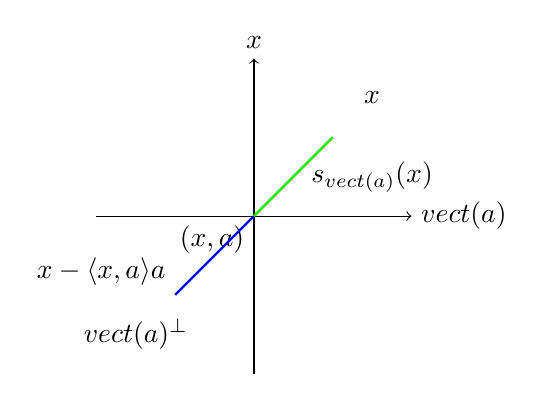
\begin{tikzpicture}
\draw[->] (-2,0) -- (2,0) node[right] {$\text{vect}(a)$};
\draw[->] (0,-2) -- (0,2) node[above] {$x$};
\draw[red, thick] (0,0) -- (1,1);
\node[below left] at (0,0) {$(x,a)$};
\node at (1.5,1.5) {$x$};
\draw[blue, thick] (0,0) -- (-1,-1);
\node[above left] at (-1,-1) {$x - \langle x, a \rangle a$};
\node at (-1.5,-1.5) {$\text{vect}(a)^\perp$};
\draw[green, thick] (0,0) -- (1,1);
\node at (1.5,0.5) {$s_{\text{vect}(a)}(x)$};
\end{tikzpicture}
\end{center}

FIGURE 2 – Réflexion orthogonale

---

III Matrices orthogonales

1 Définitions, propriétés

Définition 9. Une matrice $A \in \mathcal{M}_n(\mathbb{R})$ est dite orthogonale si elle vérifie $A^T A = I_n$.

Notations : On note $\mathcal{O}_n(\mathbb{R})$ l'ensemble des matrices orthogonales de $\mathcal{M}_n(\mathbb{R})$.

Proposition 14. Soit $A \in \mathcal{M}_n(\mathbb{R})$. On a
\[
A \in \mathcal{O}_n(\mathbb{R}) \quad \Leftrightarrow \quad A \in GL_n(\mathbb{R}) \text{ et } A^{-1} = A^T
\]
Démonstration. Propriété du groupe $GL_n(\mathbb{R})$.

Remarque : D'après les propriétés de structure de groupe de $GL_n(\mathbb{R})$, on a
\[
A^T A = I_n \quad \Leftrightarrow \quad A A^T = I_n \quad \Leftrightarrow \quad A T A = A A T = I_n
\]

B. Landelle \hspace{1cm} 7 \hspace{3cm} ISM MP

% Source image: page_008.png

Théorème 5. Soit $A \in M_n(\mathbb{R})$. Les conditions suivantes sont équivalentes :

1. $A \in O_n(\mathbb{R})$;
2. Les vecteurs colonnes de $A$ forment une base orthonormée de $\mathbb{R}^n$;
3. Les vecteurs lignes de $A$ forment une base orthonormée de $\mathbb{R}^n$.

Démonstration. Notons $(C_1, \dots, C_n)$ les colonnes de $A$. On a

\[ \forall (i,j) \in \{1, \dots, n\}^2, \quad (A^T A)_{i,j} = \sum_{k=1}^n a_{k,i} a_{k,j} = (C_i, C_j) \]

On en déduit l'équivalence (1) $\Leftrightarrow$ (2). L'équivalence (1) $\Leftrightarrow$ (3) s'en déduit par transposition car $A \in O_n(\mathbb{R}) \Leftrightarrow A^T \in O_n(\mathbb{R})$.

Remarque : On peut généraliser le sens du calcul auxiliaire vu précédemment. Pour $A = (A_1, \dots, A_n)$ et $B = (B_1, \dots, B_n)$ matrices de $M_{p,n}(\mathbb{R})$, on a $A^T B = (A_i, B_j)_{1 \leq i,j \leq n}$.

Proposition 15. Soient $\mathcal{B}_1$ une base orthonormée de $E$ et $\mathcal{B}_2$ une famille de $n$ vecteurs de $E$. On a

\[ \text{mat}_{\mathcal{B}_1}(\mathcal{B}_2) = O_n(\mathbb{R}) \Leftrightarrow \mathcal{B}_2 \text{ base orthonormée de } E \]

Démonstration. Notons $\mathcal{B}_2 = (\varepsilon_1)_{1 \leq k \leq n}$ et $P = \text{mat}_{\mathcal{B}_1}(\mathcal{B}_2) = (p_{i,j})_{1 \leq i,j \leq n}$. On a

\[ \forall (i,j) \in \{1, \dots, n\}^2, \quad (P^T P)_{i,j} = \sum_{k=1}^n p_{k,i} p_{k,j} = (\varepsilon_i, \varepsilon_j) \]

d'où

\[ P^T P = I_n \Leftrightarrow \forall (i,j) \in \{1, \dots, n\}^2, \quad (\varepsilon_i, \varepsilon_j) = \delta_{i,j} \]

\section{2 Groupe orthogonal}

Proposition 16. L'ensemble $O_n(\mathbb{R})$ est un sous-groupe de $(GL_n(\mathbb{R}), \times)$.

Démonstration. On a $I_n \in O_n(\mathbb{R})$. Soient $A, B$ dans $O_n(\mathbb{R})$. Alors $(AB)^T AB = I_n$ et $(A^{-1})^T A^{-1} = I_n$.

Définition 17. L'ensemble $O_n(\mathbb{R})$ est appelé groupe orthogonal d'ordre $n$ sur $\mathbb{R}$.

Proposition 17. Soit $A \in O_n(\mathbb{R})$. On a det $A \in \{ \pm 1 \}$.

Démonstration. On a

\[ \det(A^T A) = \det(A)^2 = \det(I_n) = 1 \]

Le résultat suit.

\textbf{Avertissement :} ce résultat ne caractérise nullement les matrices orthogonales. Pour $n \geq 2$, une matrice $A \in M_n(\mathbb{R})$ ayant un déterminant égal à 1 mais n'est pas orthogonale puisque sa dernière colonne n'est pas normée.

Définition 18. On désigne par $SO_n(\mathbb{R})$ le sous-groupe des matrices orthogonales de déterminant positif, c'est-à-dire telles que $\det A = 1$.

Proposition 19. Soient $A \in SO_n(\mathbb{R})$ et $B \in O_n(\mathbb{R})$. Alors $AB \in SO_n(\mathbb{R})$ si et seulement si $B \in SO_n(\mathbb{R})$.

Démonstration.  Si $A, B \in SO_n(\mathbb{R})$, alors $\det(AB) = \det(A) \det(B) = 1 \times 1 = 1$.

Démonstration. Soit $\varphi : O_n(\mathbb{R}) \to \{-1, 1\}$ définie par $\det(M)$. Les couples $(O_n(\mathbb{R}), \times)$ et $(-1, 1), \times)$ sont des groupes et l'application $\varphi$ est un morphisme de groupes. Alors, on a $\frac{SO(n)}{O(n)} \cong \text{Ker} \varphi$ sous-groupe de $O_n(\mathbb{R})$ comme noyau d'un morphisme de groupes. \hfill $\square$

Définition 12. L'ensemble $SO_n(\mathbb{R})$ est appelé groupe spécial orthogonal d'ordre $n$ sur $\mathbb{R}$.

Notations : On note $O_n(\mathbb{R})$ ou $O(n)$ l'ensemble des matrices orthogonales négatives.

\section{Isométries vectorielles et matrices orthogonales}

Théorème 6. Soit $u \in \mathcal{L}(E)$ et $\mathcal{B}$ une base orthonormée de $E$. On a
\[ u \in O(E) \iff \text{mat}_{\mathcal{B}} u \in O_n(\mathbb{R}) \]

Démonstration. On note $\mathcal{B} = (e_1, ..., e_n)$ et $A = \text{mat}_{\mathcal{B}} u$. On reprend les notations du théorème 5. On a
\[ \forall (x, j) \in [1; n]^2 \quad (A^T A)_{i,j} = (C_i, C_j)_{R} = \langle u(e_i), u(e_j) \rangle \]
Le résultat suit d'après le théorème 3. \hfill $\square$

Corollaire 1. Soit $A \in O_n(\mathbb{R})$. L'endomorphisme $u \in \mathcal{L}(\mathbb{R}^n)$ canoniquement associé à $A$ appartient à $O(\mathbb{R}^n)$.

Démonstration. La base canonique $\mathcal{E}$ est une base orthonormée de $E = \mathbb{R}^n$ (pour le produit scalaire canonique). Ainsi, l'endomorphisme $u \in \mathcal{L}(E)$ canoniquement associé est tel que $\text{mat}_{\mathcal{E}} u = O_n(\mathbb{R})$ d'où $u \in O(\mathbb{R}^n)$ d'après le théorème 6. \hfill $\square$

Corollaire 2. Soit $u \in \mathcal{L}(E)$ et $\mathcal{B}$ base orthonormée de $E$. On a
\[ u \in SO(E) \iff \text{mat}_{\mathcal{B}} u \in SO_n(\mathbb{R}) \]

Démonstration. Immédiate car det $u = \text{det mat}_{\mathcal{B}} u$ avec $\mathcal{B}$ base de $E$.

Remarque : On peut annoncer le même résultat en remplaçant $SO(E)$ et $SO_n(\mathbb{R})$ par $O^+(E)$ et $O_n^+(\mathbb{R})$.

\section{Réduction des isométries}

\subsection{Orientation d'un espace vectoriel}

Définition 13. Soit $\mathcal{B}$ une base de $E$. On dit qu'une base $\mathcal{B}'$ de $E$ donne la même orientation à $E$ que $\mathcal{B}$ si $\text{det}_{\mathcal{B}, \mathcal{B}'} = 1$ ou donne une orientation opposée à celle de $\mathcal{B}$ si $\text{det}_{\mathcal{B}, \mathcal{B}'} = -1$.

Définition 14. L'espace $E$ est dit orienté si on fixe une base $\mathcal{B}_0$ pour le choix de l'orientation de toute base. Une base ayant la même orientation que $\mathcal{B}_0$ est dite directe et indirecte dans le cas contraire.

Exemples : 1. $\mathbb{R}^n$ est équipé de la base canonique $\mathcal{E}$ (et donc de l'orientation qu'elle donne à $\mathbb{R}^n$). 2. $\mathbb{R}^2$ et $\mathbb{R}^3$ sont orientés.

% Source image: page_010.png

\begin{figure}[h!]
    \centering
    \includegraphics[width=\textwidth]{figure3.png}
    \caption{FIGURE 3 -- Orientation des espaces $\mathbb{R}^2$ et $\mathbb{R}^3$}
\end{figure}

\textbf{Proposition 19.} Soit $E$ espace euclidien orienté et $\mathcal{B}_1, \mathcal{B}_2$ deux bases directes de $E$. Alors on a $\det_{\mathcal{B}_1} \mathcal{B}_2 > 0$.

\textit{Démonstration.} Soit $\mathcal{B}_0$ la base de $E$ déterminant l'orientation de toute base. On a
\[
\det_{\mathcal{B}_0} \mathcal{B}_1 = \det_{\mathcal{B}_0} \mathcal{B}_2 \det_{\mathcal{B}_1} \mathcal{B}_2 = (\det_{\mathcal{B}_0} \mathcal{B}_1)^{-1} \det_{\mathcal{B}_1} \mathcal{B}_2 > 0
\]
\hfill $\square$

\textbf{Proposition 20.} Soit $E$ espace euclidien orienté et $\mathcal{B}_1, \mathcal{B}_2$ deux bases orthonormées directes de $E$. On a $\det_{\mathcal{B}_1} \mathcal{B}_2 = 1$.

\textit{Démonstration.} Soit $\mathcal{L}$ une famille de $n$ vecteurs de $E$. On a
\[
\det_{\mathcal{B}_1} \mathcal{L} = \det_{\mathcal{B}_2} \mathcal{L}
\]
et la matrice $\mathrm{Mat}_{\mathcal{B}_1} \mathcal{B}_2$ est orthogonale comme matrice de passage entre deux bases orthonormées et positive car les bases sont directes.
\hfill $\square$

\section{2 Le groupe $O_2(\mathbb{R})$}

\textbf{Théorème 7.} Soit $A \in \mathcal{M}_2(\mathbb{R})$. On a $A \in O_2(\mathbb{R})$ si et seulement s'il existe $\theta \in \mathbb{R}$ tel que
\[
A = \begin{pmatrix}
\cos \theta & -\sin \theta \\
\sin \theta & \cos \theta
\end{pmatrix}
\quad \text{ou} \quad
A = \begin{pmatrix}
\cos \theta & \sin \theta \\
\sin \theta & -\cos \theta
\end{pmatrix}
\]

\textit{Démonstration.} On pose $A = \begin{pmatrix} a & b \\ c & d \end{pmatrix}$ avec $a, b, c, d$ réels et on écrit
\[
A^T A = I_2 \iff
\begin{cases}
a^2 + c^2 = 1 \\
b^2 + d^2 = 1 \\
ab + cd = 0
\end{cases}
\iff \exists (\theta, \phi) \in \mathbb{R}^2 :
\begin{cases}
a + ic = e^{i\theta} \\
d + ib = e^{i\phi} \\
\sin(\theta + \phi) = 0
\end{cases}
\]
et comme $\sin(\theta + \phi) = 0$ équivaut à $\theta + \phi = 0 [\pi]$, on conclut par élimination de $\theta'$.\[
A A^T = I_2 \iff \exists \theta \in \mathbb{R} :
\begin{cases}
a + ic = e^{i\theta} \\
d + ic = e^{-i\theta}
\end{cases}
\quad \text{ou} \quad
e^{i(\theta+\pi)}
\]

\textbf{Corollaire 3.}
\[
SO(2,\mathbb{R}) = \{R(\theta) = \begin{pmatrix}
\cos \theta & -\sin \theta \\
\sin \theta & \cos \theta
\end{pmatrix}, \theta \in \mathbb{R}\}
\]
\[
O_2(\mathbb{R}) = \{S(\theta) = \begin{pmatrix}
\cos \theta & \sin \theta \\
\sin \theta & -\cos \theta
\end{pmatrix}, \theta \in \mathbb{R}\}
\]

B. Landelle \hfill 10 \hfill ISM MP

% Source image: page_011.png

Démonstration. Immédiate par le calcul du déterminant.

Remarque : Pour $\theta$ réel, on a $R(\theta)$ orthogonalement semblable à $R(-\theta)$. Pour $r \in \mathcal{L}(\mathbb{R}^2)$ canoniquement associé, il suffit de considérer $mat_{\sigma} \mathcal{B} = (\cos \theta, -\sin \theta; \sin \theta, \cos \theta)$ (ce qui change l'orientation de la base).

Théorème 8. L'application $R : \mathbb{R} \rightarrow SO_2(\mathbb{R})$, $\theta \mapsto R(\theta)$ est un morphisme du groupe $(\mathbb{R}, +)$ vers le groupe $(SO_2(\mathbb{R}), \times)$, autrement dit

\[
\forall (\theta, \alpha) \in \mathbb{R}^2 \quad R(\theta + \alpha) = R(\theta)R(\alpha)
\]

C'est un morphisme surjectif de noyau Ker $R = 2\pi \mathbb{Z}$ et le couple $(SO_2(\mathbb{R}), \times)$ est un groupe commutatif.

Démonstration. On sait que $SO_2(\mathbb{R})$ est un sous-groupe de $O_2(\mathbb{R})$. Le calcul donne $R(\theta)R(\alpha) = R(\theta + \alpha)$ pour tout $(\alpha, \theta) \in \mathbb{R}^2$ ce qui prouve que l'application $R$ est bien un morphisme de groupes et que la loi $\times$ est commutative sur $SO_2(\mathbb{R})$. Ce morphisme est surjectif d'après la description de $SO_2(\mathbb{R})$ faite au corollaire 3 et pour $\theta$ réel

\[
\varphi(\theta) = 1 \Leftrightarrow \theta \in 2\pi \mathbb{Z}
\]

Remarque : En particulier, pour $\theta$ réel, on a $R(\theta)^{-1} = R(-\theta)$ puisque $I_2 = R(\theta - \theta) = R(\theta)R(-\theta)$.

Corollaire 4. Soit $E$ espace euclidien orienté de dimension 2. Soit $r \in E$. Alors il existe $\theta$ réel unique modulo $2\pi$ tel que, pour toute base orthonormée directe $\mathcal{B}$, on a $mat_{\mathcal{B}} r = R(\theta)$.

Démonstration. Soit $r \in E$ et $\mathcal{B}$ une base orthonormée directe. D'après le corollaire 2, on a $mat_{\mathcal{B}} r \in SO_2(\mathbb{R})$ et d'après le corollaire 3, il existe $\theta$ réel tel que $mat_{\mathcal{B}} r = R(\theta)$ et pour $\theta'$ réel, on a $R(\theta') = R(\theta)$ si et seulement si $\theta' \equiv \theta [2\pi]$. Soit $\mathcal{B}'$ une base orthonormée directe de $E$. D'après la proposition 15, on a $P = mat_{\mathcal{B}'} \mathcal{B} \in O_2(\mathbb{R})$ et comme les deux bases sont directes, on a det $P > 0$ donc $P \in SO_2(\mathbb{R})$ et par suite, $P = R(\alpha)$ avec $\alpha \in \mathbb{R}$. Ainsi, d'après les formules de changement de base

\[
mat_{\mathcal{B}'} r = P mat_{\mathcal{B}} r P^{-1} = R(\alpha) R(\theta) R(-\alpha) = R(\theta)
\]

Démonstration 15. Soit $E$ un espace vectoriel réel de dimension finie. Soient $\mathcal{B}$ et $\mathcal{B}'$ deux bases orthonormées directes de $E$. La matrice de passage de la base $\mathcal{B}$ vers la base $\mathcal{B}'$ est une matrice $P$ telle que pour tout vecteur $r$ de $E$, on a $mat_{\mathcal{B}'} r = P mat_{\mathcal{B}} r$. On a $P^{-1} = mat_{\mathcal{B}} \mathcal{B}'$ et on a det $P = \pm 1$. Si les bases sont directes, alors det $P = 1$ et $P \in SO_n(\mathbb{R})$.

Remarque : Une base orthonormée directe de $E$ est une base $(e_1, \dots, e_n)$ de $E$ qui est orthonormée et telle que le déterminant de la matrice dont les colonnes sont les coordonnées de $e_1, \dots, e_n$ dans une base quelconque est positif.

Proposition 16. Soit $E$ un espace euclidien orienté de dimension $n$. Soit $\mathcal{B} = (e_1, \dots, e_n)$ une base orthonormée directe de $E$. Alors l'application $r \mapsto mat_{\mathcal{B}} r$ est un isomorphisme de $E$ vers $\mathcal{M}_n(\mathbb{R})$.

Démonstration. Soit $r \in E$. Alors $r = \sum_{i=1}^n \langle r, e_i \rangle e_i$. Donc $mat_{\mathcal{B}} r = (\langle r, e_1 \rangle, \dots, \langle r, e_n \rangle)^t$. L'application est donc bien définie. Elle est linéaire car l'application $r \mapsto \langle r, e_i \rangle$ est linéaire.

\[
\forall r \in E, \quad r = 0 \Leftrightarrow \forall i \in \{1, \dots, n\}, \langle r, e_i \rangle = 0 \Leftrightarrow mat_{\mathcal{B}} r = 0
\]

Donc l'application est injective.

% Source image: page_012.png

\textbf{Définition 16.} Soit $E$ euclidien orienté de dimension 2 et $\vec{u}, \vec{v}$ deux vecteurs non nuls de $E$.
On appelle mesure de l'angle orienté d'un couple de vecteurs $(\vec{u}, \vec{v})$ une mesure $\theta$ de l'angle
de l'unique rotation qui transforme $\vec{u}$ en $\vec{v}$, que l'on note $(\vec{u}, \vec{v})$, définie modulo $2\pi$
par :
\[ (\vec{u}, \vec{v}) \equiv \theta [2\pi] \]
Illustration d'une rotation $r \in SO(\mathbb{R}^2)$ d'angle
$\theta$ réel.

\begin{figure}[H]
\centering
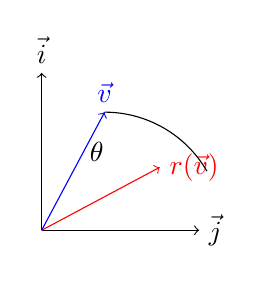
\begin{tikzpicture}
\draw[->] (0,0) -- (2,0) node[right] {$\vec{j}$};
\draw[->] (0,0) -- (0,2) node[above] {$\vec{i}$};
\draw[->, red] (0,0) -- (1.5,0.8) node[right] {$r(\vec{v})$};
\draw[->, blue] (0,0) -- (0.8,1.5) node[above] {$\vec{v}$};
\draw (0.8,1.5) arc (90:30:1.5);
\node at (0.7,1) {$\theta$};
\end{tikzpicture}
\caption{FIGURE 4 – Rotation dans $\mathbb{R}^2$}
\end{figure}

\textbf{Théorème 10.} Soit $E$ euclidien de dimension 2 et $s \in O(E)$. Alors $s$ est une symétrie
orthogonale et il existe une base orthonormée $\mathcal{B}$ telle que $mat_{\mathcal{B}} s = \begin{pmatrix} 1 & 0 \\ 0 & -1 \end{pmatrix}$.

\textit{Démonstration.} Soit $\mathcal{B}'$ base orthonormée de $E$. Alors $mat_{\mathcal{B}'} s( \theta)$ avec $\theta$ réel. On a $S(\theta)^2 = I_d$ et donc $s$ symétrie et $s \in O(E)$ donc $s$ est une symétrie orthogonale. On a clairement
$s \neq \pm id$ car $S(\theta) \neq \pm I_2$ ou car det $s = 1$. Il en résulte $E = \text{Ker}(s - id) \oplus \text{Ker}(s + id)$
où chacun des sev de la décomposition est une droite vectorielle. En considérant une base
orthonormée $\mathcal{B}$ adaptée à cette décomposition, on a $mat_{\mathcal{B}} s = \text{diag}(1, -1)$.
$\square$

\textbf{Remarque :} Les éléments de $O_2(\mathbb{R})$ sont des matrices de réflexions.

Illustration d'une réflexion $s \in O^-(\mathbb{R}^2)$ avec
$\mathcal{B} = (e_1, e_2)$ une base de réduction.

\begin{figure}[H]
\centering
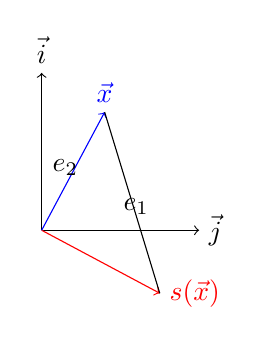
\begin{tikzpicture}
\draw[->] (0,0) -- (2,0) node[right] {$\vec{j}$};
\draw[->] (0,0) -- (0,2) node[above] {$\vec{i}$};
\draw[->, red] (0,0) -- (1.5,-0.8) node[right] {$s(\vec{x})$};
\draw[->, blue] (0,0) -- (0.8,1.5) node[above] {$\vec{x}$};
\draw (0.8,1.5) -- (1.5,-0.8);
\node at (1.2,0.3) {$e_1$};
\node at (0.3,0.8) {$e_2$};
\end{tikzpicture}
\caption{FIGURE 5 – Réflexion dans $\mathbb{R}^2$}
\end{figure}

B. Landelle \hspace{2cm} 12 \hspace{5cm} ISM MP
% Source image: page_013.png

\section{3 Réduction d'une isométrie}

\textbf{Proposition 21.} Soit $u \in O(E)$ et $F$ sev de $E$ stable par $u$. L'endomorphisme induit $u_F$ est une isométrie de $F$.

\textit{Démonstration.} Immédiate. \hfill $\square$

\textbf{Proposition 22.} Soit $u \in O(E)$ et $F$ sev de $E$ stable par $u$. Alors $F^\perp$ est stable par $u$.

On commence par énoncer le lemme suivant :

\textbf{Lemme 1.} Soit $E$ un $\mathbb{K}$-ev de dimension finie, $u \in GL(E)$ et $F$ sev de $E$ stable par $u$. Alors, on a $u(F) = F$.

\textit{Démonstration.} On applique le théorème du rang à $u$ et le résultat suit.

\textit{Démonstration de la proposition 21.} D'après le lemme, on a donc $u(F) = F$. Soit $(x, y) \in F^\perp \times F$. Comme $F = u(F)$, il existe $z \in F$ tel que $y = u(z)$ d'où
\[ (u(x), y) = (u(x), u(z)) = (x, z) = 0 \]
On en déduit $u(F^\perp) \subseteq F^\perp$ ce qui prouve le résultat attendu.

\textit{Variante.} On peut aussi utiliser le fait que $F^\perp$ est stable par $u^\ast$. Comme $u \in O(E)$, on a $u^\ast = u^{-1}$ et d'après le lemme, on obtient $u^{-1}(F^\perp) = F^\perp$ puis $u(u^{-1}(F^\perp)) = u(F^\perp)$ autrement dit $F^\perp = u(F^\perp)$.

\textbf{Remarque :} Les inclusions $u(F) \subset F$ et $u(F^\perp) \subset F^\perp$ sont en fait des égalités.

\textbf{Théorème 11.} Soit $u \in O(E)$. Il existe une base orthonormée $\mathcal{B}$ de $E$ telle que la matrice mat$_\mathcal{B} u$ soit diagonale par blocs avec des blocs diagonaux de la forme
\[ \begin{pmatrix} -1 & 0 \\ 0 & 1 \end{pmatrix} \quad \begin{pmatrix} \cos \theta & -\sin \theta \\ \sin \theta & \cos \theta \end{pmatrix} \quad \theta \in \mathbb{R} \]

\textit{Démonstration.} On procède par récurrence forte sur $n = \dim E$. Le cas $n = 1$ est immédiat et le cas $n = 2$ résulte de ce qui précède. Supposons le résultat vrai jusqu'à $n - 1 \geq 2$ fixé. Soit $u \in O(E)$ avec $\dim E = n$.

\begin{itemize}
    \item Si $u$ admet une valeur propre, on considère $x$ un vecteur propre normé associé. On a $u(x) = \lambda x$. Comme $F = \text{Vect}(x)$ est stable par $u$, alors $F^\perp$ également et on applique l'hypothèse de récurrence à l'endomorphisme $u_{F^\perp}$. On obtient un système de base orthonormée de $F^\perp$ dans lequel la matrice de $u_{F^\perp}$ est diagonale.
    \item Supposons que $u$ n'a pas de valeur propre. Alors, $\text{mat}_\mathcal{B} u$ est de la forme $\begin{pmatrix} 0 & -1 \\ 1 & 0 \end{pmatrix}$. Soit $F = \text{Vect}(x_1, x_2)$ un plan invariante par $u$ tel que $u(x_1) = x_2$ et $u(x_2) = -x_1$. On pose $x_1 = e_1$ et $x_2 = e_2$. Alors, $F^\perp$ est stable par $u$ et $\dim F^\perp = n - 2$. On applique l'hypothèse de récurrence à $u_{F^\perp}$.
\end{itemize}

\textbf{Exemple 1.} Soit $u \in O(\mathbb{R}^3)$ une rotation d'angle $\theta$ autour de l'axe $\mathcal{D}$ engendré par $e_3$. Alors, dans la base $\mathcal{B} = (e_1, e_2, e_3)$, la matrice de $u$ est
\[ \begin{pmatrix} \cos \theta & -\sin \theta & 0 \\ \sin \theta & \cos \theta & 0 \\ 0 & 0 & 1 \end{pmatrix} \]

\textbf{Exemple 2.} Soit $u : \mathbb{R}^3 \to \mathbb{R}^3$ définie par $u(x, y, z) = (x, y, -z)$.

% Source image: page_014.png

Il s'ensuit $(\alpha - i\beta, \alpha + i\beta) = (0,0) \Leftrightarrow \begin{pmatrix} 1 & -i \\ 1 & i \end{pmatrix} \begin{pmatrix} \alpha \\ \beta \end{pmatrix} = \begin{pmatrix} 0 \\ 0 \end{pmatrix} \Leftrightarrow (\alpha, \beta) = (0,0)$.

Par conséquent, la famille $(X_1, X_2) = \left( \frac{X+X}{2}, \frac{X-X}{2} \right)$ est libre. Or, on a

$AX = \lambda X \Leftrightarrow AX_1 + iAX_2 = (\alpha X_1 - \beta X_2) + i(\beta X_1 + \alpha X_2) \Leftrightarrow \begin{cases} AX_1 = \alpha X_1 - \beta X_2 \\ AX_2 = \beta X_1 + \alpha X_2 \end{cases}$.

Ceci prouve l'existence d'un plan vectoriel $F$ stable par $u$. Comme $F^{\perp}$ est stable par $u$, on applique l'hypothèse de récurrence à $u_{|F}$ et $u_{|F^{\perp}}$ et la concaténation des bases donne le résultat souhaité.

Variante. On suppose que $u$ n'admet pas de valeur propre. Le polynôme caractéristique se décompose en produit de facteurs irréductibles de $\mathbb{R}[X]$ de degré 2. Il existe donc un facteur $P_1(u)$ de cette décomposition tel que $P_1(u) \in GL(E)$, sinon on aurait $x_1(u) \in GL(E)$ alors que $x_1(u) = 0$. Ainsi, il existe $a, b$ réels et $x \in \mathbb{R}^n$ tels que $(u^2 + au + b)x = 0$, c'est-à-dire $u^2(x) = -au(x) - bx$. Par conséquent, l'espace $Vect(x, u(x))$ est stable par $u$. C'est un plan vectoriel car sinon, on aurait $(r, u(x))$ liée d'où $u(x) = \lambda x$ avec $\lambda$ un réel ce qui est exclu. On conclut comme précédemment.

Corollaire 5. Soit $E$ euclidien orienté de dimension 3 et $r \in SO(E)$. Alors il existe une base orthonormée directe $\mathcal{B}$ et $\theta \in \mathbb{R}$ tels que

$mat_{\mathcal{B}} r = \begin{pmatrix} 1 & 0 & 0 \\ 0 & \cos \theta & -\sin \theta \\ 0 & \sin \theta & \cos \theta \end{pmatrix}$.

Démonstration. Soit $r \in SO(E)$. D'après le théorème de réduction d'une isométrie, il existe une base $\mathcal{B}$ orthonormée telle que $mat_{\mathcal{B}} r$ est diagonale par blocs, formée de $(1), (-1)$ ou $(\mathbb{R}(\theta))$. Si $mat_{\mathcal{B}} r$ est formée de (1) ou (-1), comme $r \in SO(E)$, alors on a $mat_{\mathcal{B}} r = I_3$ ou $mat_{\mathcal{B}} r = diag(1, -1, -1)$ quitte à réordonner $\mathcal{B}$. Ces cas correspondent aux situations où $r$ est l'identité. Sinon, le matrice $mat_{\mathcal{B}} r$ n'est pas diagonale et comme $r \in SO(E)$, on a $mat_{\mathcal{B}} r = \begin{pmatrix} 1 & 0 & 0 \\ 0 & \cos \theta & -\sin \theta \\ 0 & \sin \theta & \cos \theta \end{pmatrix}$ quitte à réordonner $\mathcal{B}$. Enfin, quitte à opposer le premier vecteur de la base, on peut choisir $\theta$ directement.

Corollaire 6. Soit $A \in SO_3(\mathbb{R})$. Il existe $\begin{pmatrix} \theta \\ \vec{u} \end{pmatrix} \in \mathbb{R} \times \mathbb{R}^3$ tel que

$mat_{\mathcal{B}} A = \begin{pmatrix} 1 & 0 & 0 \\ 0 & \cos \theta & -\sin \theta \\ 0 & \sin \theta & \cos \theta \end{pmatrix}$,

où $\mathcal{B}$ est une base orthonormée directe et $\vec{u}$ est l'axe de rotation de $A$. En particulier, si $A$ est une rotation d'angle $\theta$ autour de l'axe $\vec{u}$, alors $tr(A) = 1 + 2\cos \theta$.

Application. On calcule facilement l'expression analytique de $r$ dans $\mathbb{R}^3$. Soit $\mathcal{B} = (e_1, e_2, e_3)$ une base orthonormée directe de $\mathbb{R}^3$. On a

$r(e_1) = e_1$, $r(e_2) = \cos \theta e_2 - \sin \theta e_3$, $r(e_3) = \sin \theta e_2 + \cos \theta e_3$.

Exemple. Soit $r$ la rotation de $60^{\circ}$ autour de l'axe $Oz$. Alors $\theta = \frac{\pi}{3}$ et $r(x, y, z) = (x, \frac{y}{2} - \frac{\sqrt{3}}{2} z, \frac{y\sqrt{3}}{2} + \frac{z}{2})$.

Remarque. On peut écrire $r$ sous la forme $r = \begin{pmatrix} 1 & 0 & 0 \\ 0 & \cos \theta & -\sin \theta \\ 0 & \sin \theta & \cos \theta \end{pmatrix}$.

% Source image: page_015.png

Remarque : Comme $r \neq \text{id}$, on a $\theta \neq [2\pi]$ et $x_r = (X-1)(X - e^{i\theta})(X - e^{-i\theta})$ scindé dans $\mathbb{C}$ avec 1 racine simple d'où $\text{dim}(E_r) = 1$.

Illustration : Soit $x \in E$. On décompose $x = y + z$ avec $(y, z) \in \text{Ker}(r - \text{id}) \times \text{Ker}(r - \text{id})^\perp$.

\begin{center}
\includegraphics[width=0.8\textwidth]{image.png}
\end{center}

FIGURE 6 – Rotation $r = \text{rot}(a, \theta)$

Remarque : L'axe $\text{Ker}(r - \text{id})$ et l'angle $\theta$ ne suffisent pas à caractériser la rotation. En effet, si on prend — au lieu de $a$, il faut effectuer une rotation d'angle $-\theta$ pour effectuer la même transformation. D'où la nécessité de préciser un vecteur et un angle pour une rotation donnée.

Remarque « culturelle » : Soit $E = \mathbb{R}^3$ euclidien orienté. On suppose $a$ normé. On a
\[
\forall x \in E \quad r(x) = (1 - \cos \theta) \frac{a \wedge x}{||a||^2} + \cos \theta x + \sin \theta (a \wedge x)
\]
Retrouvons cette formule. Pour $x \in E$, on a
\[
x = y + z \quad \text{avec} \quad y = (x, a) a = \text{Pv}_{\text{vect}(a)}(x) \quad \text{et} \quad z = x - (x, a) a
\]
Par suite
\[
r(x) = r(y) + r(z) = y + r(z)
\]

B. Landelle \hfill 15 \hfill ISM MP
% Source image: page_016.png

\begin{figure}[h]
    \centering
    \includegraphics[width=0.5\textwidth]{figure7.png}
    \caption{FIGURE 7 -- Rotation rot($\alpha$, $\theta$)}
\end{figure}

En remarquant que la famille $(a, \alpha, z)$ est orthogonale directe avec $\|z\| = \| \alpha \|$, on obtient
\[
r(z) = \cos \theta z + \sin \theta (\alpha \wedge z)
\]
\[
= \cos \theta (x - (x,a)a) + \sin \theta [\alpha \wedge (x - (x,a)a)]
\]
\[
r(z) = \cos \theta (x - (x,a)a) + \sin \theta (\alpha \wedge x)
\]

V Endomorphismes auto-adjoints

Une matrice $M \in \mathcal{M}_n(\mathbb{R})$ est dite symétrique si elle vérifie $M = M^T$ ou de manière équivalente $m_{ij} = m_{ji}$ pour tout $(i,j) \in \{1, \dots, n\}^2$. On note $\mathcal{S}_n(\mathbb{R})$ l'ensemble des matrices symétriques de $\mathcal{M}_n(\mathbb{R})$. L'ensemble $\mathcal{S}_n(\mathbb{R})$ est un sev de $\mathcal{M}_n(\mathbb{R})$, par exemple en écrivant $\mathcal{S}_n(\mathbb{R}) = \text{Ker } \varphi$ avec $\varphi : M \mapsto M - M^T$ clairement linéaire. Pour $M \in \mathcal{S}_n(\mathbb{R})$, on peut écrire
\[
M = \sum_{1 \leq i < j \leq n} m_{ij} E_{ij} = \sum_{1 \leq i < j \leq n} \frac{m_{ij} - m_{ji}}{2} (E_{ij} + E_{ji})
\]
\[
\in \mathcal{S}_n(\mathbb{R})
\]
La famille $(E_{ij} + E_{ji})_{1 \leq i < j \leq n}$ est donc génératrice de $\mathcal{S}_n(\mathbb{R})$ et libre donc forme une base de $\mathcal{S}_n(\mathbb{R})$.

1 Définition

Définition 18. Soit $u \in \mathcal{L}(E)$. L'endomorphisme $u$ est dit auto-adjoint si $u = u^*$, c'est-à-dire
\[
\forall (x, y) \in E^2 \quad \langle u(x), y \rangle = \langle x, u(y) \rangle
\]

Vocabulaire : On dit aussi que $u$ est un endomorphisme symétrique.

Notations : On note $\mathcal{F}(E)$ l'ensemble des endomorphismes auto-adjoints.

Proposition 23. L'ensemble $\mathcal{F}(E)$ est un sev de $\mathcal{L}(E)$.

Démonstration. On a $0_{E} \in \mathcal{F}(E)$ puis, pour $(\lambda, \mu, u, v) \in \mathbb{R} \times \mathcal{F}(E)^2$, on a
\[
\forall (x, y) \in E^2 \quad \langle (\lambda u + \mu v)(x), y \rangle = \lambda \langle u(x), y \rangle + \mu \langle v(x), y \rangle
\]
\[
= \lambda \langle x, u(y) \rangle + \mu \langle x, v(y) \rangle = \langle x, (\lambda u + \mu v)(y) \rangle
\]
donc $\lambda u + \mu v \in \mathcal{F}(E)$.

\hfill $\square$

B. Landelle \hspace{2cm} 16 \hspace{2cm} ISM MP
% Source image: page_017.png

\textbf{Proposition 24.} Soit $u \in \mathcal{L}(E)$ et $\mathcal{B}$ une base orthonormée de $E$. On a
\[ u \in \mathcal{E}(E) \iff \text{nat}_{u} \in \mathcal{Z}(\mathbb{R}) \]
\textit{Démonstration.} (1) $\Rightarrow$ (2) Pour tout $(i,j) \in \{1; n\}^2$, on a $(u(e_j), e_i) = (e_i, u(e_j))$ d'où le résultat.
(2) $\Rightarrow$ (1) Soit $(x,y) \in E^2$. On a
\[ (u(x), y) = \sum_{j=1}^n \langle x, u(e_j) \rangle y_j = \sum_{j=1}^n x_j y_j \langle u(e_j), e_j \rangle = \dots \]
Remarque : Soit $S \in \mathcal{L}(\mathbb{R})$ et $u \in \mathcal{Z}(\mathbb{R})$ canoniquement associé à $S$. Alors $u \in \mathcal{E}(\mathbb{R}^n)$
$\mathcal{E}$ base canonique est une base orthonormée de $\mathbb{R}^n$ pour le produit scalaire canonique.

\textbf{2 Propriétés}

\textbf{Proposition 25.} Soit $p$ un projecteur de $E$. On a
\[ p \text{ projecteur orthogonal } \iff p \in \mathcal{E}(E) \]
\textit{Démonstration.} Soit $p$ projecteur orthogonal et $(x,y) \in E^2$. On a
\[ (p(x), y) = (p(x), p(y)) + (p(x), y - p(y)) = (p(x), p(y)) \]
expression symétrique en $x$ et $y$ d'où le résultat. Supposons $p \in \mathcal{E}(E)$. On a
\[ \forall (x,y) \in \text{Ker } p \times \text{Im } p \quad (x,y) = \langle x, p(y) \rangle = (p(x), y) = 0 \]
d'où le résultat. On a utilisé l'égalité $\text{Im } p = \text{Ker } (id - p)$. $\square$

\textbf{Proposition 26.} Soit $u \in \mathcal{L}(E)$ et soient $\lambda_1 \in \text{Sp}(u)$ avec $\lambda_1 \neq 0$. On a $u(x) \in \text{Ker}(u)$.
\textit{Démonstration.} Soit $(x,y) \in E \times E$ et $(u(x)) \times E$. On a
\[ \lambda (x,y) = (u(x), y) = (x, u(y)) = u(x,y) \iff \lambda \neq 0 \quad (x, u(y)) = 0 \iff x \perp y \]

\textbf{Proposition 27.} Soit $u \in \mathcal{L}(E)$ et $F$ un sev stable par $u$. Alors l'endomorphisme induit $u_F$ est un endomorphisme auto-adjoint de $F$.
\textit{Démonstration.} Immédiate.

\textbf{Proposition 28.} Soit $u \in \mathcal{L}(E)$ et $F$ un sev stable par $u$. Alors $F^{\perp}$ est stable par $u$.
\textit{Démonstration.} Conséquence immédiate de la proposition 4. $\square$

\vspace{1cm}
B. Landelle \hspace{2cm} 17 \hspace{2cm} ISM MP

\section{Théorème spectral}

\textbf{Théorème 12.} Soit $u \in \mathcal{E}(E)$. Alors $u$ admet une valeur propre.

\textit{Démonstration.} Soit $B$ une base orthonormale de $E$ et $M = \text{mat}_{\mathcal{B}}(u)$. On a $M \in \mathcal{M}_n(\mathbb{R})$. Soit $\lambda$ une racine de $\chi_M$ dans $\mathbb{C}$. Soit $X \in \mathbb{C}^n$ non nul tel que $MX = \lambda X$. En conjuguant puis en multipliant à gauche par $X^*$, on trouve $X^*MX = \lambda X^*X$. Puis partant de $MX = \lambda X$, en transposant puis en multipliant par $X$ à droite, on trouve $X^*MX = \lambda X^*X$. Comme $X^*X > 0$, il s'ensuit par identification que $\lambda = \lambda$, autrement dit $\lambda$ racine réelle de $\chi_M = X_\mu$ d'où le résultat.

\textbf{Théorème 13 (Théorème spectral).} Soit $u \in \mathcal{E}(E)$. Alors
\[
E = \bigoplus_{\lambda \in \text{Sp}(u)} E_\lambda(u)
\]
ou, de manière équivalente, il existe une base orthonormée de vecteurs propres de $u$.

\textit{Démonstration.} Soit $F = \bigoplus_{\lambda \in \text{Sp}(u)} E_\lambda(u)$ sev non réduit à $\{0_E\}$ d'après le théorème précédent. On vérifie sans difficulté que $F$ est stable par $u$. Supposons $F^\perp \neq \{0_E\}$. On a $F^\perp$ stable par $u$ et l'endomorphisme induit par $u$ sur $F^\perp$ est symétrique donc admet un vecteur propre qui l'est aussi pour $u$. On aurait alors $F \cap F^\perp$ non réduit à $\{0_E\}$ ce qui est absurde. La décomposition équivaut à l'existence d'une base orthonormée de vecteurs propres de $u$. Pour le sens direct, il suffit de considérer une base orthonormée adaptée à la décomposition. Pour le sens indirect, on a la décomposition souhaitée par diagonalisation et celle-ci est orthogonale car $u$ est symétrique.

\textit{Variante :} On peut aussi, par récurrence forte sur $n = \dim E$, prouver l'existence d'une base orthonormée de vecteurs propres. Il suffit en effet de concaténer des bases orthonormées de vecteurs propres pour $u_E$ et $u_{F^\perp}$ avec $F = E_\lambda(u)$ (si $F \neq E$ rien à faire), les vecteurs propres pour ces endomorphismes induits étant aussi vecteurs propres pour $u$.

\textbf{Corollaire 7.} Soit $A \in \mathcal{M}_n(\mathbb{R})$. Il existe $P \in O_n(R)$ et $D \in \mathcal{M}_n(\mathbb{R})$ diagonale telles que
\[
P^{-1}AP = D
\]

\textit{Démonstration.} La base canonique est une base orthonormée. D'après le théorème spectral, il existe une base orthonormée $(u_1, \dots, u_n)$ de vecteurs propres de $A$ pour laquelle la matrice de $A$ est diagonale. Soit $P$ la matrice de passage de la base canonique à la base $(u_1, \dots, u_n)$. Alors $P^{-1}AP$ est diagonale et $P^{-1}AP = D$ où $D$ est la matrice diagonale dont les coefficients sont les valeurs propres de $A$. Comme $P$ est une matrice de passage d'une base orthonormée à une autre, $P$ est orthogonale, donc $P \in O_n(R)$.

\textbf{Remarque :} On dit que $A$ est diagonalisable orthogonale.

\textbf{Définition 8.} Soit $E$ un $\mathbb{R}$-espace vectoriel muni d'un produit scalaire. Un endomorphisme $u$ de $E$ est dit orthogonal si $\langle u(x), y \rangle = \langle x, u(y) \rangle$ pour tous $x, y \in E$.

% Source image: page_019.png

\section{VI Positivité}

\subsection{1 Définitions}

Définition 19. Soit $u \in \mathcal{L}(E)$. L'endomorphisme $u$ est dit positif si
\[
\forall x \in E, \quad (u(x),x) \geq 0
\]
L'endomorphisme $u$ est dit défini positif si
\[
\forall x \in E \setminus \{0\}, \quad (u(x),x) > 0
\]
Notations : On note $\mathcal{P}^{+}(E)$ l'ensemble des endomorphismes auto-adjoints positifs de $E$ et
$\mathcal{P}^{++}(E)$ l'ensemble des endomorphismes auto-adjoints définis positifs de $E$.

Définition 20. Soit $M \in \mathcal{M}_n(\mathbb{R})$. La matrice $M$ est dite positive si
\[
\forall X \in \mathcal{M}_n(\mathbb{R}), \quad (MX,X) \geq 0
\]
La matrice $M$ est dite définie positive si
\[
\forall X \in \mathcal{M}_n(\mathbb{R}) \setminus \{0\}, \quad (MX,X) > 0
\]
Notations : On note $\mathcal{S}_n^{+}(\mathbb{R})$ l'ensemble des matrices symétriques positives et $\mathcal{S}_n^{++}(\mathbb{R})$ l'ensemble des matrices symétriques définies positives.

Remarque : Le calcul donne $(MX,X) = X^T MX = \sum_{1 \leq i,j \leq n} x_i x_j m_{ij}$.

Proposition 29. Soit $u \in \mathcal{L}(E)$ et $\mathcal{B}$ une base orthonormée de $E$. On a
\[
u \in \mathcal{P}^{+}(E) \Leftrightarrow \text{mat}_{\mathcal{B}} u \in \mathcal{S}_n^{+}(\mathbb{R})
\]
\[
u \in \mathcal{P}^{++}(E) \Leftrightarrow \text{mat}_{\mathcal{B}} u \in \mathcal{S}_n^{++}(\mathbb{R})
\]
Démonstration. On sait que $u \in \mathcal{L}(E)$ et $\text{mat}_{\mathcal{B}} u \in \mathcal{S}_n(\mathbb{R})$. L'équivalence pour le caractère positif ou défini positif est immédiate.

\subsection{2 Propriétés}

Les résultats qui suivent sont déclinés vectoriellement mais existent à l'identique en version matricielle.

Proposition 30. Soit $u \in \mathcal{L}(E)$, $\mathcal{B} = (e_1, \dots, e_n)$ une base orthonormée de vecteurs propres de $u$ associés aux valeurs propres $\lambda_1, \dots, \lambda_n$ (répétées avec multiplicité) et $x = \sum_{i=1}^n x_i e_i \in E$. On a
\[
(u(x),x) = \sum_{i=1}^n \lambda_i x_i^2
\]
Avec $E = \bigoplus_{i \in \mathcal{A}} E_{\lambda_i}(u)$ et $x = \sum_{i \in \mathcal{A}} x_i$ la décomposition associée, on a
\[
(u(x),x) = \sum_{i \in \mathcal{A}} ||x_i||^2
\]

B. Landelle
\hspace{1cm}
19
\hspace{1cm}
ISM MP

% Source image: page_020.png

Démonstration. On a
\[
(u(x), x) = \sum_{i \leq j \leq n} x_{ij} (u(e_i), e_j) = \sum_{i \leq j \leq n} \lambda_{ij} (e_i, e_j) = \sum_{i=1}^n \lambda_{ii}
\]
Avec la décomposition orthogonale $x = \sum_{\lambda \in \text{Sp}(u)} x_\lambda$, il vient
\[
(u(x), x) = \sum_{(\lambda, \mu) \in \text{Sp}(u)^2} (u(x_\lambda), x_\mu) = \sum_{(\lambda, \mu) \in \text{Sp}(u)^2} \langle \lambda x_\lambda, x_\mu \rangle = \sum_{\lambda \in \text{Sp}(u)} \lambda |x_\lambda|^2
\]
Remarque : Pour la version matricielle, on considère $P \in \mathcal{O}_n(\mathbb{R})$ telle que $P^\top MP = D$ diagonale. Ainsi, pour $X$ et $Y$ dans $\mathbb{C}_n(\mathbb{R})$ avec $X = PY$, on a
\[
(MX, X) = X^\top M^\top X = Y^\top D^\top Y = \sum_{i=1}^n \lambda_i^2
\]
Théorème 14. Soit $u \in \mathcal{F}(\mathbb{E})$. On a
\[
u \in \mathcal{F}^+(\mathbb{E}) \Leftrightarrow \text{Sp}(u) \subset [0; +\infty[
\]
et
\[
u \in \mathcal{F}^{++}(\mathbb{E}) \Leftrightarrow \text{Sp}(u) \subset ]0; +\infty[
\]
Démonstration. Pour $\lambda \in \text{Sp}(u)$ et $x \in E_\lambda(u)$ qu'on choisit normé, il vient
\[
(u(x), x) = \lambda \geq 0 \text{ si } u \in \mathcal{F}^+(\mathbb{E}) \text{ et } > 0 \text{ si } u \in \mathcal{F}^{++}(\mathbb{E})
\]
Réciproquement, si $\text{Sp}(u) \subset [0; +\infty[$, l'expression obtenue à la proposition 30 permet d'établir $(u(x), x) \geq 0$ pour $x \in \mathbb{E}$. Si $\text{Sp}(u) \subset ]0; +\infty[$ et $x \in \mathbb{E} \setminus \{0\}$, une de ces coordonnées $x_\lambda$ est non nulle et on en déduit $(u(x), x) > 0$.

Théorème 15 (À savoir refaire). Soit $u \in \mathcal{F}(\mathbb{E})$ et $\lambda_1 < \dots < \lambda_n$ les valeurs propres de $u$. On a
\[
\forall x \in \mathbb{E} \qquad \frac{\Vert x \Vert^2}{\lambda_n} \leq \langle u(x), x \rangle \leq \Vert x \Vert^2
\]
et si une des inégalités est une égalité avec $x$ non nul, alors $x$ est vecteur propre.

Démonstration. Soit $\mathcal{B} = (e_1, \dots, e_n)$ base orthonormée de vecteurs propres associés à $\lambda_1, \dots, \lambda_n$ et $x \in \mathbb{E}$ avec $x = \sum_{i=1}^n x_i e_i$ réels et aussi $x = \sum_{\lambda \in \text{Sp}(u)} x_\lambda$ avec $x_\lambda \in E_\lambda(u)$ pour $\lambda \in \text{Sp}(u)$. D'après la première expression obtenue dans la proposition 30, on a
\[
\langle u(x), x \rangle = \sum_{i=1}^n \lambda_i x_i^2
\]
et d'après la deuxième l'encadrement. Supposons $\langle u(x), x \rangle = \lambda_n \Vert x \Vert^2$ de la proposition 30,
\[
\langle u(x), x \rangle = \sum_{\lambda \in \text{Sp}(u)} \lambda |x_\lambda|^2 = \lambda_n \sum_{\lambda \in \text{Sp}(u)} |x_\lambda|^2
\]
ce qui implique $\lambda = \lambda_n$ pour tout $\lambda \in \text{Sp}(u)$ et donc $x \in E_{\lambda_n}(u)$.

ISM 1992

% Source image: page_021.png

\section*{Annexe}

\subsection*{Génération aléatoire d'une matrice orthogonale}

On présente en langage python un procédé pour générer aléatoirement une matrice orthogonale.

La fonction pa(A,B) d'arguments A, B deux matrices de $M_n(\mathbb{R})$ renvoie $(A, B) = \sum_{i \leq j, k \leq n} a_{i,j,k}$
et la fonction isortho(A) d'argument A une matrice de $M_n(\mathbb{R})$ renvoie True si la matrice A est orthogonale et False sinon.

\begin{verbatim}
def pa(A,B):
    return np.trace(A.T.dot(B))

def isortho(A):
    eps=1e-8
    B=A.T.dot(A)-np.eye(len(A))
    return ps(B,B)<eps
\end{verbatim}

On rappelle l'algorithme d'orthonormalisation de Gram-Schmidt :

\textbf{Algorithme 1} Orthonormalisation

\textbf{ENTRÉES:} $\{u_1, ..., u_p\}$ libre

\textbf{SORTIES:} $\{v_1, ..., v_p\}$ orthonormée

\begin{itemize}
    \item res $\leftarrow u_1/||u_1||$
    \item pour $k \in \{2: p\}$ faire
    \item \quad $z \leftarrow u_k - \sum_{i=1}^{k-1} (u_k, v_i) v_i$
    \item \quad res $\leftarrow$ res $+ \frac{z}{||z||}$
    \item fin pour
    \item renvoie res
\end{itemize}

Dans l'algorithme, l'étape itérative consiste à construire $z_k = u_k - P_k(u_k)$ où
$F_k = \text{Vect} \{u_1, ..., u_{k-1}\} = \text{Vect} \{v_1, ..., v_{k-1}\}$.

Ainsi, on a
\[
u_k \leftarrow \frac{z_k}{||z_k||} \quad \text{d'où} \quad v_k \perp u_i \quad \forall i \in [1: k-1]
\]

\begin{center}
\includegraphics[width=0.8\textwidth]{figure8.png}
\end{center}

FIGURE 8 – Étape itérative de l'algorithme d'orthonormalisation

\vspace{1cm}

B. Landelle \hfill 21 \hfill ISM MP
% Source image: page_022.png

Une implémentation de l'algorithme est donnée par :

\begin{verbatim}
def norm(u) :
  # normalise le vecteur u
  return u/alg.norm(u)

def ortho(A) :
  # Renvoie la matrice constituée des colonnes orthonormalisées
  # à partir des colonnes de la matrice A
  p=A.shape[1]
  v=[norm(A[:,0])]
  for k in range(1,p):
    u=A[:,k]
    z=sum([np.dot(v[i],u)*v[i] for i in range(k)])
    v.append(norm(u-z))
  return np.array(v).T
\end{verbatim}

On remarque que l'implémentation d'une fonction de normalisation qui prend un vecteur en entrée et le normalise rend la fonction ortho très lisible avec une écriture assez légère.

On applique l'algorithme d'orthonormalisation aux colonnes d'une matrice $A \in \mathcal{M}_p(\mathbb{R})$ de rang égal à $p$ (avec $p \leq n$) transmise en argument. Si $p = n$, la famille orthonormalisée $(v_1, \dots, v_n)$ est une base orthonormée de $\mathbb{R}^n$. Ainsi, on peut facilement générer aléatoirement une matrice orthogonale par orthonormalisation d'une matrice tirée aléatoirement dans $GL_n(\mathbb{R})$ :

\begin{verbatim}
>>> A=rd.rand(3,3)
>>> B=ortho(A)
>>> np.dot(B.T,B)
array([[ 1.00000000e+00,  5.05754733e-15, -8.89543056e-15],
       [ 5.05754733e-15,  1.00000000e+00, -1.03875092e-15],
       [-8.92318613e-15, -1.03875092e-15,  1.00000000e+00]])
>>> isortho(B)
True
\end{verbatim}

B. Landelle
22
ISM MP
\end{document}